
% Tento soubor nahraďte vlastním souborem s obsahem práce.
%=========================================================================
% Autoři: Michal Bidlo, Bohuslav Křena, Jaroslav Dytrych, Petr Veigend a Adam Herout 2019

\chapter{Úvod}
\label{uvod}
Tato diplomová práce se zabývá volumetrickým vykreslováním sněhových útvarů známých jako kajícníci (en. penitentes). S primárním zaměřením na co možná nejvěrnější vyobrazení průchodu světla těmito útvary. Pro vykreslování těchto útvarů bude v rámci této práce implementována metoda \textit{Progressive Transient Photon Beams}\cite{ptpb}.

Diplomová práce se bude zabývat i odvozením optických vlastností útvarů typu kajícník. Pro tuto práci je nutné tato data získat. Vzhledem k tomu, že se nepodařilo  dohledat žádné volně dostupné soubory optických dat pro vykreslování kajícníkům  či alespoň sněhu nebo sněhových struktur, bude potřeba čerpat z fyzikálních prací zabývajících se touto tématikou. 

Bohužel prací zabývajících se přímo kajícník je minimálně, a žádná se nezabývá přímo jejich optickými vlastnostmi. V diplomové práci je tedy nutné mimo jiné čerpat z prací studujících glaciální led v Dómu C na Antarktidě\cite{refinement_ice}\cite{snow_properties}, dále pak z prací zabývající se sněhem obecně\cite{soos} a z dalších pracích o sněhové pokrývce, primárně v Antarktidě.

Existuje mnoho metod pro volumetrické vykreslování příkladem může být uvedeno \textit{Photon mapping}, \textit{Ray marching}, \textit{volumetrick bidirectional path tracing}, \textit{beam radiance estimate} a~další. V  této diplomové práci budou v rámci teorie popsány metody \textit{Photon mapping}, \textit{Photon beams} a \textit{Transient photon beams} neboť metoda \textit{Progressive Transient Photon Beams} jež bude implementována pro vizualizaci práce na výše zmíněné metody navazuje. Zvolení metody předcházelo testování vykreslování modelu kajícníka pomocí \textit{SmallUPBP}\cite{smallubpb}.  Metoda \textit{Progressive Transient Photon Beams} byla vybrána na základě testů, které proběhly se srovnatelnými výsledky při užití různých typů metod viz \ref{porovnani1} a~\ref{porovnani2}. Jedná se tedy o metodu, která typově není zastoupena ve \textit{SmallUPBP}. Tato metoda se~od~ostatních odlišuje mimo jiné i tím, že nepředpokládá, že světlo se šíří nekonečně rychle. To znamená, že se tedy paprsek z kamery musí s tímto světelným paprskem potkat jak prostorově, tak i časově.

Přínos této práce spočívá v zjištění vhodných metod pro vykreslování sněhových a ledových struktur, primárně tedy kajícníků. Dále ve~zkompletování optických vlastností sněhu pro volumetrické vykreslování. Vykreslování těchto struktur může být použito v mnoha odvětvích počítačové grafiky. Vzhledem k tomu, že se jedná o krásné a netradiční útvary, které mohou ozvláštnit mnoho vykreslovaných scenérií. V neposlední řadě je přínosem této práce i vytvoření volné implementace \textit{Progressive Transient Photon Beams} (žádnou jinou se do~současnosti nepodařilo dohledat). 

\chapter{Výběr metody}
\section{Vykreslování sněhu}
Sníh je materiál o mnoha podobách, dle toho se můžou diametrálně lišit vhodné metody pro jeho vykreslování. Kromě vlastní podoby sněhu záleží i~na~tom, kde a za jakým účelem bude sníh vykreslován. Cesta sněhu začíná v~podobě padajících částic. Tyto částice bude nejvhodnější vykreslovat pomocí částicových efektů. K napadané sněhové pokrývce, která může měnit svoji výšku zejména v čase, se~dá přistupovat několika různými úhly pohledu. Pracovat se sněhovou pokrývkou tedy můžeme jako s~kapalinou, pevným objektem či jako s velkým množstvím částic. Dále je možné postupovat až k sedlému sněhu měnícího se v~led, respektive sněhové struktury typu koulí, sněhuláků či kajícníků, které jsou již nutně pevnými objekty. Pro~každou podobu jsou pak vhodné jiné metody. Například sněhovou pokrývkou se zabývá práce \textit{Real-time Rendering of Accumulated Snow}\cite{accumulated-snow} nebo padajícím sněhem se~zabývá práce \textit{A~Modeling and Rendering Method for Snow by Using Metaballs}\cite{falling-snow2}, případně \textit{A~Spectral-particle hybrid method for rendering falling snow}\cite{falling-snow}.

Zatímco padajícím sněhem či sněhovou pokrývkou se~zabývá hodně prací, přece jen se jedná o velmi časté jevy, tak~sněhovým strukturám zas tolik pozornosti věnováno není. A~to~zejména proto, že~se~k~vykreslení padajícího sněhu a sněhových pokrývek dá využít realističnosti, fyzikální přesnosti i realtimového vykreslování. Sněhové struktury jsou přece jen až na sněhuláky vzácnější, případně se jedná o~lokální úkazy. Proto pro výběr vhodné metody bylo provedeno testování vícero možných metod, vhodných k vykreslování sněhových struktur.

\section{Různé metody} \label{ruz-met}
Na obrázcích v této kapitole je všude stejný model vygenerovaný pomocí práce Ondřeje Čecha\cite{FITBT22558}. K vykreslování byly použity metody implementované ve \textit{SmallUPBP}\cite{smallubpb} pomocí dávkového souboru \textit{run\_reference\_snow.bat} ze scény \textit{snow} přiložené ke kódu práce. V~prvním kroku porovnávání metod byly všechny metody spuštěny po dobu jedné hodiny. V~tomto intervalu se u většiny metod nedostaneme k příliš kvalitním výsledkům. Tento krok však postačí k vyřazení metod, které výrazně zaostávají. Všechny metody pomocí, kterých byly následující obrázky vyrendrovány jsou volumetrické. 

\begin{figure}[H]\centering

\includegraphics[width=0.5\linewidth]{obrazky-figures/reference_upbp_surf_3600.png}\hfill
\includegraphics[width=0.5\linewidth]{obrazky-figures/reference_upbp_pp3d_3600.png}\hfill
  \caption{\textbf{Metody \textit{Surface photon mapping} a \textit{Medium photon mapping} s 3D kernelem}}
  \label{porovnani1}
\end{figure}
\begin{figure}[H]\centering
\includegraphics[width=0.5\linewidth]{obrazky-figures/reference_upbp_bpm_3600.png}\hfill
\includegraphics[width=0.5\linewidth]{obrazky-figures/reference_upbp_bb1d_3600.png}\hfill
  \caption{\textbf{Metody \textit{Bidirectional photon mapping} a  \textit{Photon beams} s 1D kernelem}}
  \label{porovnani2}
\end{figure}
\begin{figure}[H]\centering
\includegraphics[width=0.5\linewidth]{obrazky-figures/reference_upbp_ptmis_3600.png}\hfill
\includegraphics[width=0.5\linewidth]{obrazky-figures/reference_upbp_ptls_3600.png}\hfill
  \caption{\textbf{Metody\textit{Path tracing MIS} a \textit{Path tracing with light sampling}}}
  \label{porovnani3}
\end{figure}
\begin{figure}[H]\centering
\includegraphics[width=0.5\linewidth]{obrazky-figures/reference_upbp_pb2d_3600.png}\hfill
\includegraphics[width=0.5\linewidth]{obrazky-figures/reference_upbp_bpt_3600.png}\hfill
  \caption{\textbf{Metody \textit{BRE (beam vs points)} s 2D kerlnelem a \textit{Bidirectional path tracing (BPT)}}}
  \label{porovnani4}
\end{figure}
\newpage
Kromě výběru vhodné metody, by v práci měla být i implementována metoda, která je popsána ve vědeckém článku bez volně dostupné implementace. Cílem tohoto testování je vybrat vhodný typ metody. Jak je vidět na obrázcích \ref{porovnani4}, tak metody \textit{Volumetric biderctional path tracing (BPT)} a BRE s 2D kernelem mají kvalitativně srovnatelné výsledky. Proto byly hledány metody vycházející z \textit{photon beamů} nebo BPT. Nejzajímavější z nalezených byla metoda \textit{Progresive Transient Photon Beams}\cite{ptpb}, která by díky iterativnímu přístupu měla dosahovat stejných výsledků, ale s menšími nároky na paměť. Dále díky využití prostorového i časového kernelu by měla dosahovat realističtějších výsledků.  

\chapter{Progressive transient photon beams}
\label{teorie-vr}
% prehled metod, porovnani vhodnosti, seznam co potřebuji pro rendering
V této kapitole bude popsána teorie týkající se metody \textit{Progressive Transient Photon Beams} a dále pak i základní metody ze kterých tato metoda vychází. Konkrétně se bude jednat o~\textit{Photon mapping, Photon beams} a~\textit{Transient photon beams}. Anglické slovo "\textit{beam}"~užívané v~této práci, má v češtině pouze jediný ekvivalent a to "paprsek", což je~zde ovšem nadmíru nedostatečné. Zejména proto, že v~rámci vykreslovacích metod je paprsek vžit jako "ray", tedy jako \textit{ray tracing}. Mezi~\textit{ray} a \textit{beam} je při užití v dané problematice značný významový rozdíl. \textit{Ray} přestavuje paprsek o nulové ploše řezu (geometricky úsečka), zatím co \textit{beam} představuje spíše svazek paprsků. Jeho řez má nenulovou plochu, z výpočetního hlediska se jedná o~válec, proto je v této diplomové práci slovo "\textit{beam}" ponecháno ve~svém původním anglickém jazyce a není nepřekládáno, ale počešťováno.      
\section{Photon mapping}\label{pm}
Při užití metody \textit{Photon mapping} se paprsky vrhají jak z kamery, tak~ze~zdrojů světla. Metoda funguje na principu uplatňovaní dvou kroků. V~prvním kroku metody se vrhají paprsky ze zdrojů světla a výsledky se~ukládají do fotonové mapy. Ve~druhém kroku se provádí \textit{ray tracing} z kamery. Osvětlenost bodů dopadů paprsků z~kamery se počítá na~základě údajů, které jsou uloženy ve fotonové mapě.
\subsection{První krok}
Zdroj světla vygeneruje dané množství fotonů. Tyto fotony se pohybují směrem ze zdroje, což se samozřejmě odvíjí od typu světelného zdroje. Jestliže dojde k dopadu na rozhraní materiálů, může nastat jedna ze dvou situací (viz níže), které jsou většinou voleny náhodně nebo na základě pravděpodobnosti. Pravděpodobnost je vypočítána na základě koeficientu zániku daného materiálu.\\
\\ 
Situace:
\begin{enumerate}
    \item foton zanikne
    \item dojde k odrazu či lomu a foton pokračuje dál 
\end{enumerate}
\\ 
Jestliže foton nezanikl, je na základě \textit{BRDF} (\textit{Bidirectional reflectance distribution function}) funkce určen jeho nový směr a energie\cite{photon_mapping}.\\ 

\textit{BRDF} funkce definuje tři typy odrazu:
\begin{enumerate}
   \item Difuzní odraz -> záznam do fotonové mapy (místo dopadu, příchozí směr, světelný tok)
    \item lesklý odraz -> foton pokračuje dál
    \item lom do materiálu -> pokračuje dál materiálem
\end{enumerate}
 
 \subsection{Druhý krok}
V druhém kroku se pomocí \textit{ray tracingu} vykresluje výsledný obraz. Rozdílem oproti klasickému \textit{ray tracingu} je v tom, že~osvětlenost bodu se počítá pomocí údajů ve fotonové mapě a to dle rovnice \ref{pm_eq}. Bod~dopadu paprsku je x ze směru $\omega$.

\begin{equation}\label{pm_eq}
    L_r(x,\vec{\omega}) \approx \frac{1}{\pi r^2} \sum_{p=1}^{N}f(x,\vec{\omega},\vec{\omega}_p)\Delta\phi_p(x,\vec{\omega}_p)
\end{equation}
Kde $\frac{1}{\pi r^2}$ představuje velikost okolí, ze kterého jsou vybírány záznamy ve fotonové mapě. N~je~počet fotonů (bodů dopadů z prvního kroku) v okolí bodu x. $f$ může být opět \textit{BRDF} nebo \textit{BSDF} či~jiná fázová funkce, která vrátí koeficient přispění fotonu $p$. $\phi$ je velikost světelného toku fotonu $p$.
\section{Photon beams}
Tento algoritmus je prezentován v článku \textit{A Comprehensive Theory of Volumetric Radiance Estimation Using Photon Points and Beams}\cite{comprehensive}. Rozšiřuje algoritmus \textit{Photon mapping}, mimo~jiné tím, že nahrazuje fotonovou mapu \textit{Photon beams map}. \textit{Photon beams map} ukládá při~interakci fotonu s prostředím opět bod, směr a světelný tok. Zatím co v metodě \textit{Photon mapping} se do mapy ukládají body, tedy místa dopadů fotonů, v metodě \textit{Photon beams} jsou ukládány \textit{beamy}. \textit{Beam} není bod, ale je to prostor, konkrétně válec, definovaný letem fotonu od místa vzniku/odrazu/lomu až k místu dopadu.

V druhém kroku algoritmu se stejně jako v metodě \textit{Photon mapping} sledují paprsky z~kamery, ale osvětlenost místa dopadu se počítá na základě protnutých \textit{beamů} jako suma příspěvku všech protnutých paprsků. Je-li tedy paprsek z kamery definován jako $x_r + s_r \vec{\omega}_r$, kdy $x_r$ je místo dopadu paprsku, $s_r$ jeho délka a $\vec{\omega}_r$ směr odkud přichází, tak rovnice \ref{pB} vyjadřuje míru osvětlenosti bodu x na základě toho paprsku.\\
\begin{equation}\label{pB}
    L(x_r \xleftarrow[]{} \vec{\omega}_r,s) \approx \frac{\sigma_s}{\mu_r(r^2)}\sum_{b \in R_b} L_b(x_r \xleftarrow[]{}  \vec{\omega}_r, s).
\end{equation}
Kde $\sigma_s$ je koeficient pro rozptyl v daném mediu, $\mu_r(r^2)$ je~velikost oblasti (pro 2D kernel je $\mu_r(r^2)$ = $\pi(r^2)$). Následná suma je přes všechny \textit{beamy}, které paprsek z kamery po cestě k bodu dopadu protne. Vliv jednoho \textit{beamu} na ovsvětlení bodu x ze směru $\omega$ lze vyjádřit rovnicí \ref{Lb}:\\
 \begin{equation}\label{Lb}
    L_b(x_r \xleftarrow[]{}\omega_c,s) = f(\theta_b)\Phi_b\int_{t_b^-}^{t_b^+}e^{\sigma_t t_b}e^{\sigma_t t_c}dt_b
\end{equation}
Kde $f(\theta_b)$ je fázová funkce a $\theta_b$ je úhel mezi \textit{beamem} a paprskem z kamery. Dále $\Phi_b$ je~velikost světelného toku daného \textit{beamu}. Integrál od $t_b^-$ do je $t_b^+$ vyjadřuje míru přispění daného \textit{beamu} a představuje plochu protnutí viz obrázek \ref{2d}. $\sigma_t$ je koeficient pohlcení a  $t_b$ respktive $t_c$ jsou body průniku. Podle $t_b$ je integrováno a $t_c$ je možné z~$t_b$ odvodit dle rovnice \ref{tbtc}.
 \begin{equation}\label{tbtc}
    t_c = t_c^- - |\cos(\theta_b)|(t_b - t_b^-),
\end{equation}
Kdy $t_c^-$ je skalární projekcí $t_b^-$.
Rovnice \ref{Lb} i \ref{pB} počítají s takzvaným 2D \textit{kernelem}. Vliv~\textit{beamu} na paprsek je potom odvozen od plochy čtyřúhelníku, viz obrázek \ref{2d}. Dále je možné používat i 1D či 3D kernel. 1D kernel uvažuje vzdálenost paprsku z kamery a paprsku definující \textit{beam} ve~středu úsečky tvořené vstupním a výstupním bodem paprsku z kamery do~prostoru \textit{beamu}. 3D kernel bude objem generovaný vstupními a výstupními body podobně jako plocha 2D kernelu. Rovnice pro 1D a 3D se mírně liší (pro 3D je o integrál složitější a pro 1D jednoduší). Jejich přesné tvary je možné dohledat v článku \cite{comprehensive}, odkud jsou čerpány i všechny rovnice v této podkapitole.

\begin{figure}[h]\centering
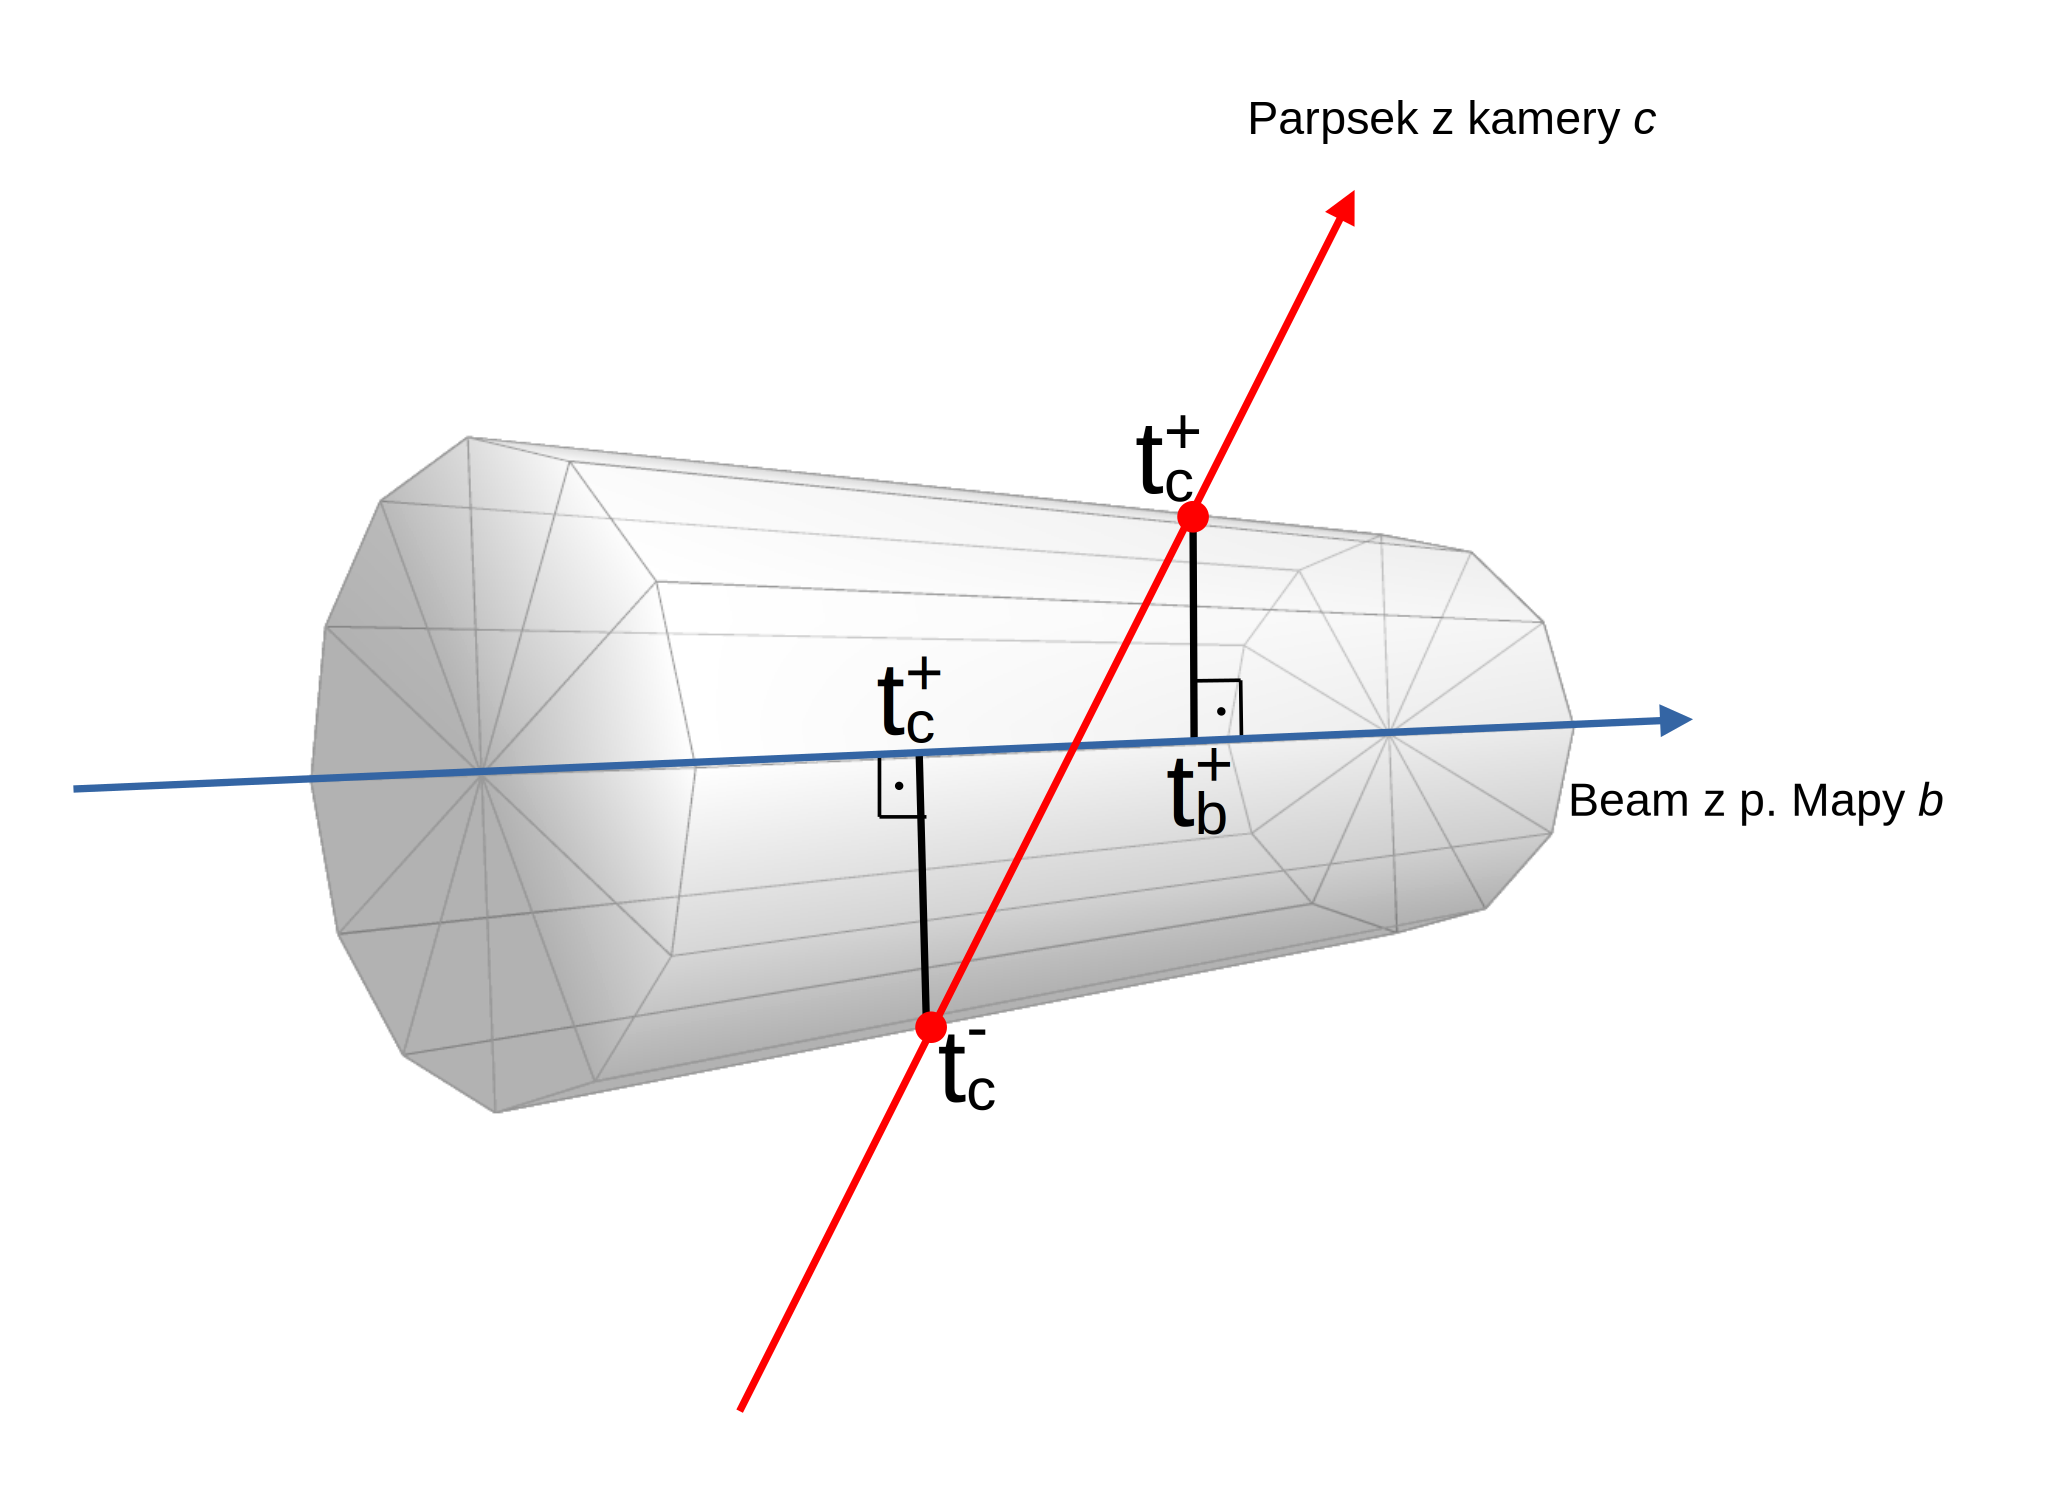
\includegraphics[width=0.7\linewidth]{obrazky-figures/2DKernel.png}\hfill
  \caption{\textbf{2D kernel}}
  \label{2d}
\end{figure}
\section{Transient photon beams} 
\textit{Transient photon beams}\cite{transient_pb} je rozšíření standardního algoritmu \textit{photon beams} o~dobu letu jednotlivých fotonů. Světlo se totiž pohybuje různou rychlostí, v závislosti na rozdílných materiálech. Zásadním rozdílem oproti \textit{stedy-state} variantě je, že kromě místa, směru a~světelného toku také to, že se do~\textit{Photon beam map} musí ukládat ještě čas, kdy tam fotony dorazily. V čase $t$ se začnou vrhat fotony ze zdrojů světla a při každém záznamu do fotonové mapy se vypočítá čas letu.
Druhý krok začíná opět v čase $t$, při výpočtu vlivu jednotlivých \textit{beamů} je zahrnut doba letu fotonu i~paprsku k danému místu.  
Rovnice pro \textit{estimator}\footnote{\textit{Estimator} je úsek kódu, odhadující množství světla dopadajícího na daný bod z daného směru. V této kapitole bude slovo počešťováno. Vhodný překlad by mohl být odhadce, ale \textit{estimator} je zavedený pojem na rozdíl od odhadce.} bude zahrnovat další proměnou a~to~čas. To znamená, že bude vyjadřovat míru osvětlení bodu $x_r$, na který je nahlíženo ze směru $\vew(\omega_r)$ v čase $t$. Jestliže by ovšem byl využit 2D \textit{kernel} nebude se jednat o čas $t$, ale o časový interval od času vstupu do prostoru \textit{beamu} do času výstupu.
Rovnice \ref{Lbt1d} je pro 1D \textit{kernel} a  \ref{Lbt2d} pro 2D \textit{kernel}\cite{ptpb}.

 \begin{equation}\label{Lbt1d}
    L_b^{1D}(x_r,\vec{\omega_r}) = K_{1D}(R_b)\Phi_b f_s(\Theta_b)\mu_s \frac{e^{-\mu_t s_b}e^{-\mu_t s_r}}{\sin{\Theta_b}}
\end{equation} 
\begin{equation}
 \label{Lbt2d}
    L_b^{2D}(x_r,\vec{\omega_r}) = K_{2D}(R_b)\Phi_b f_s(\Theta_b)\mu_s \frac{e^{-\mu_s(s_c^--s_c+)(|\cos{\Theta_b}|-1)}-1}{e^{\mu_s(s_c^--s_b-)}\mu_t(|\cos{\Theta_b}|-1)}
\end{equation}
V rovnicích  \ref{Lbt1d} a \ref{Lbt2d} $L_b$ představuje přispění jednoho \textit{beamu} k paprsku  z $x_r$ ve směru $\vec{\omega_r}$. $R_b$ je radius \textit{beamu}, $\Phi_b$ je světelný tok, $f_s$ fázová funkce, $\Theta_b$ představuje úhel mezi \textit{beamem} a~paprskem z kamery. $\mi_s$ a $\mi_t$ jsou koeficienty media pro rozptyl a zánik. $S_b$ a $S_r$ respektive $S_b^+$/$S_b^-$ a $S_c^+$/$S_c^-$ představují hraniční body \textit{kernelu}, viz body $t$ v obrázku \ref{2d} pro 2D \textit{kernel} a v obrázku \ref{1d} pro 1D \textit{kernel}.
\section{Progressive Transient Photon Beams}
\textit{Progressive Transient Photon Beams} (dále PTPB) se od \textit{Transient photon beams} odlišuje použitím iterativního \textit{estimatoru}. Tedy \textit{estimator} v tomto případě nevrací celkový odhad světla, ale odhad světla po $n$ iteracích. Pro každou iteraci je používáno nové sady \textit{beamů}. V článku\cite{ptpb}, ze kterého tato práce čerpá informace o PTPB, je logika metody popsána pomocí pseudo-kódu, jenž je v upravené verzi uveden v algoritmu \ref{ptpb-pc}.
\begin{algorithm}[h]\label{ptpb-pc}
\SetAlgoLined
\KwResult{Míra osvětlení bodu pro paprsek r}
 $L_0 \gets 0$\;
 $R_0 \gets R_0$\;
 $\Tau \gets \Tau_0$\;
 \For{$i \in [0 \dots n]$}{
    $R \gets getAllRayFromCamera()$\;
    $B \gets beamsMap()$\;
    \For{$r \in R$}{
        $R_b \gets R_b\sqrt{\frac{i+\frac{2}{3}}{i+1}}$\;
        $\tau \gets \tau\sqrt{\frac{i+\frac{2}{3}}{i+1}}$\;
        $L_b \gets 0$\;
        $Br \gets intersects(r,B)$\;
        \For{$b \in Br$}{
            $L_b \gets L_b + radiance(r,b,R_b,\tau)$\;
        }
         $L_n[r] \gets L_n + L_b$\;
    }
 }
 \caption{Výpočet Transient photon beams}
\end{algorithm}
\newpage
Algoritmus \ref{ptpb-pc} provede $n$ iterací, kdy v každé vypočítá mapu \textit{beamů} a pro každý paprsek z~kamery zjistí jeho průniky s jednotlivými \textit{beami}. Na základě průniků potom připočte vliv \textit{beamu} k celkovému osvětlení místa dopadu paprsku $r$ pro danou iteraci.

Generování mapy je stejné jako \textit{Photon Beams} nebo \textit{Transient photon beams} metody. Přispění jednoho \textit{beamu} k osvětlení paprsku z kamery, je definován rovnicí \ref{ptpb-eq}\cite{ptpb} (výpočet radiance z algoritmu \ref{ptpb-pc}).
\begin{equation}
 \label{ptpb-eq}
    L_b^{1D}(x_r,\vec{\omega_r},t) = K_{1D}(R_b)\Phi_b f_s(\Theta_b, t)\mu_s \frac{e^{-\mu_t s_b}e^{-\mu_t s_r}}{\sin{\Theta_b}}K_\tau(t - t_b)
\end{equation}
Kde $\Phi_b$ je světelný tok \textit{beamu}. $\f_s(\Theta_b,t)$ je fázová funkce (pro různá media můžou být vhodné různé typy fázových funkcí). $\mu_t$ a $\mu_s$ jsou koeficienty pohlcení a rozptylu, $\Theta_b$ je úhel mezi parpskem z kamery a protnutým \textit{beamem}. Zbývají $\K_{1D}(R_b)$ a $\K_{\tau}(t-t_b)$, které jsou prostorovým a~časovým \textit{kernelem}. Časový kernel může být například pro 1D \textit{kernel} Dirakova delta funkce:
\begin{equation}
 \label{dirak-delta}
   \delta(x) = =\begin{cases}
    $$+ \infty$$ & $pro x = 0$\\
    0 &  $$pro x \neq 0$$
  \end{cases}
\end{equation}
Prostorový \textit{kernel} se vyskytuje již v metodě \textit{Photon beams}, na základě článku \cite{ptpb} je vhodné použít 1D prostorový \textit{kernel}, neboť nezpůsobuje rozmazání v čase. To, proto že při použití 2D nebo 3D prostorového \textit{kernelu}, časy vstupu paprsku do~prostoru \textit{beamu} a výstupu jsou různé, zatímco pro 1D \textit{kernel} se jedná o jeden bod v čase. Jako 1D prostorový \textit{kernel} je~možné použít $\frac{1}{d}$, kdy $d$ je~vzdálenost vektorů v bodě, tedy "protnutí"~viz obrázek \ref{1d}.
\begin{figure}[h]\centering
\includegraphics[width=0.5\linewidth]{obrazky-figures/1DKernel.png}\hfill
  \caption{\textbf{1D \textit{kernel}}}
  \label{1d}
\end{figure}

\chapter{Optické vlastnosti sněhu}\label{opt-snow}
Cílem práce je co nejnerealističtější vykreslování sněhu a sněhových struktur. Důležitá není tedy jenom vhodná metoda, ale i správně nastavené optické vlastnosti media. Dle práce \cite{vevoda} je potřeba u každého materiálu znát jeho albedo, absorpci, rozptyl a vyzařování. Hodnoty těchto vlastností jsou pro realistické vykreslování potřeba změřit na~skutečném sněhu. Z toho důvodu bylo čerpáno z prací měřících optické vlastni sněhové pokrývky na~Antarktidě\cite{snow_properties}\cite{refinement_ice} nebo optickými vlastnostmi sněhu obecně\cite{soos}.
U sněhu je problém, že se vyskytuje v mnoha formách: čerstvě napadlý, zledovatělý, mokrý, sedlý a v mnoha dalších. K dalším aspektům optických vlastností patří i případné znečištění prachem či jinými částicemi. Proto je potřeba si při definování vlastností modelu i ujasnit, za jakých okolností je vykreslován a za jakých případně vzniká. V této práci jsou jako model použity kajícníci, sněhová struktura vyskytující se ve výších nadmořských výškách s přímým osvitem slunce.  
\section{Kajícníci}
Jak bylo řečeno, optické vlastnosti sněhu mají velký rozsah, proto je potřeba si specifikovat o jaký typ sněhu či sněhovou strukturu se bude jednat. Pro účely této práce tak byli vybráni kajícníci. 
\begin{figure}[h]\centering
\includegraphics[width=1\linewidth]{obrazky-figures/kajinici1.jpg}\hfill
  \caption{\textbf{Kajícníci v poušti Atacama\cite{wiki_snow}}}
  \label{2d}
\end{figure}

Kajícníci jsou sněhové útvary vznikající na horských úbočích (například na území velehor And a pohoří Himalájí\cite{Betterton2000FormationOS}), v nadmořských výškách od 4000 m n. m. a výše\cite{lliboitry_1954}.  Tvarem připomínají stojící desky, které se směrem nahoru zužují. Tyto desky stojí v řadách za sebou, všechny orientované stejným směrem. Výška útvarů se pohybuje od několika desítek centimetrů až po 6 m. V nižších nadmořských výškách (3000 a více) se ještě mohou vyskytovat i mikrokajícníci. Jedná se o~velmi podobné útvary, ale rozměrově mají pouhý 1 až 15 cm. Své jméno získali díky podobnosti s klečícími (kajícími se) lidmi v bílých špičatých kápích, které se ve Španělsku či latinsko-amerických zemích nosí při církevních slavnostech.  
\begin{figure}[h]\centering
\includegraphics[width=0.6\linewidth]{obrazky-figures/penitetntsSpain.jpg}\hfill
  \caption{\textit{Penitents take part in the “Cristo de la sangre” (Christ of the Blood) procession during Holy Week celebrations in Palma de Mallorca. Foto Jamie Reina}\cite{penitentsSpain}}
  \label{2d}
\end{figure}

Ohledně fyzikální příčiny a podmínek vzniku těchto útvarů, za dobu jejich zkoumání, vzniklo mnoho různých teorií\cite{lliboitry_1954}. Posléze ale byla většina z těchto myšlenek vyvrácena v~roce 1942 Carlem Trollem. Na základě svých experimentů dokázal, že vznik souvisí primárně se sluncem. Tedy se směrem, ze kterého na danou oblast svítí, avšak přesné příčiny zatím nejsou dokázány\cite{lliboitry_1954}. Faktory potřebné ke vzniku kajícníků jsou: přímé slunce, suché studené počasí, sníh bez nečistot jak na povrchu, tak uvnitř\cite{Betterton2000FormationOS}. Kajícníci vznikají ze sněhu, jenž přes léto neroztál.
\section{Albedo}
Albedo je koeficient vyjadřující míru odrazivosti materiálu. Většinou se uvádí jako desetinné číslo v rozsahu 0 až 1, kdy jedna odráží veškeré světlo a nula žádné. V případě sněhu obecně může albedo dosahovat až 0,9, to znamená, že až 90\% světla se odrazí. Této hodnoty dosahuje zejména čerstvě napadaný sníh bez nečistot (většinou prachové částice, písek či~zemina). Jak bylo zmíněno, ve vyšších polohách kajícníci vznikají pouze za podmínky, že sněhová pokrývka neobsahuje žádné nečistoty. To znamená, že hodnota albeda v době napadnutí může dosahovat 0,9, ale sníh postupem času odrazivé vlastnosti ztrácí. V práci \textit{Scattering optics of snow}\cite{soos}, která se zabývá optickými vlastnostmi sněhových kulovitých částic, uvádí že albedo velkých sněhových částic může dosahovat až 0.89. U menších částic může hodnota albeda klesat až na 0.78. Závislost albeda na velikosti částic velmi rychle inklinuje k 0.89, proto by se při vykreslování mělo vycházet z 0.89 až 0.86, ale níže s~největší pravděpodobností nikoliv.
\section{Absorpce}
Absorpce vyjadřuje kolik světla materiál pohltí, respektive jak moc je světlo při průchodu materiálem utlumeno. \textit{Refinement of the ice absorption spectrum in the visible using radiance profile measurements in Antarctic snow}\cite{refinement_ice} se zabývá měřením světelné absorpce ledové pokrývky na Antarktidě ve vlnových délkách 320 nm až 600 nm a to v~hloubce v~rozmezí 20 - 30 cm. V této hloubce by stále mělo jednat spíše o velmi zhutnělý sníh než přímo o led. Což je tedy podobná pokrývka jako je ta, ze které se následně formují kajícníci. Většina počítačové grafiky pracuje s RGB modelem pro reprezentaci barev a světelná absorpce sněhu se pro jednotlivé vlnové délky mění, proto absorpci bude reprezentovat trojice a(r,g,b) = (0.2345, 0.04708, 0.02246). Použité vlnové délky jsou pro modrou 470 nm, zelenou 530 nm a pro červenou 640 nm. Vzhledem k tomu že naměřená data končí na~vlnové délce 600 nm, která odpovídá oranžové, tak byla hodnota pro 640 nm extrapolována z naměřených data. 
\section{Rozptyl}\label{rozptyl}
Tento koeficient popisuje jak moc se světlo při dopadu rozptýlí nebo respektive odrazí, čím je vyšší, tím více je světlo odraženo do více směrů. Dle práce \textit{Visible and near-ultraviolet absorption spectrum of ice from transmission of solar radiation into snow} \cite{snow_extiction_scattering}, kde uvádí vazbu mezi koeficientem rozptylu, absorbce a zániku (\textit{extiction}). $$ \sigma_t = \sigma_a + \sigma_s$$  Koeficient zániku lze vyčíst z grafu 1 v \textit{Snow Characterization by Optical Properties}\cite{extin1} a~z~grafu 4 v \textit{Theory of the optical properties of snow}\cite{extin2}. Vzhledem k tomu, že se jedná o~hodnoty čtené z grafu, bude pravděpodobně potřeba vyzkoušet několik různých hodnot k optimalizaci výsledku. $\sigma_t = (13, 9, 6)$ jsou hodnoty odečtené z grafu č.1 v \cite{extin1}. $\sigma_t =~(4, 1.5, 0.7)$ jsou z grafu č. 4 v \cite{extin2}, $\sigma_t = (30, 19, 8)$ jsou z grafu č. 4 v \cite{snow_extiction_scattering}. Je vidět, že naměřené hodnoty mají relativně velký rozptyl, souvisí to s různou hloubkou v jaké bylo  měření provedeno. Dále pak s různou hustotou sněhu i různou velikostí částic sněhu. Proto bude potřeba tyto hodnoty použít spíše jako výchozí body pro~testování, než jako pevné konstanty. Všechny tři sady koeficientů jsou počítány na metr tloušťky materiálu. Dále dle \cite{soos}, je možné pro nízké hodnoty absorpce aproximovat rozptyl jako zánik $\sigma_s \approx \sigma_t$, což je i~případ sněhu, neboť absorpce se pohybuje v řádu $10^{-2}$, zatímco rozptyl je v řádu $10^{1}$ až~$10^{2}$.
\section{Index lomu}
Index lomu nemá tak přímý vliv na optický vzhled objektu jako předchozí parametry, ale o~to zásadnější vliv má na pohyb paprsků ve scéně a také na rychlost jejich šíření. U většiny metod není brána v potaz rychlost šíření paprsků, proto nad ní není uvažováno, ale u \textit{PTPB}, která využívá jak prostorový, tak časový \textit{kernel} je rychlost důležitá. Bez rychlosti by nebylo možné spočítat, v jakém čase je paprsek/\textit{beam} v daném bodě. V rámci výpočtu je uplatněn Snellův zákon. $$v = \frac{c}{n}$$ 
\newpage
Kdy $v$ je výsledná rychlost světla v daném materiále, $c$ je~rychlost ve vakuu a $n$ je absolutní index lomu daného materiálu.
Index lomu sněhu se dle práce \cite{soos} pohybuje mezi 1.31 - 1.27.
\section{Vyzařování}
Vyzařování se týká pouze materiálů jenž svítí, zdrojů světla. Což není případ sněhu, proto hodnota vyzařování sněhu je logicky rgb vektor (0,0,0). 

\chapter{Návrh řešení}
Při implementaci vykreslovací metody je potřeba zajisti několik periferních funkcionalit. Příkladem to je: načítání scén, vykreslování do \textit{framebufferu}, ukládání ve vhodném formátu, struktury či třídy pro uchovávání a zpracovávání dat. Pak také několik velmi důležitých funkcionalit, jako například výpočet \textit{photon beam map}, či vyhodnocování, které paprsky a~které \textit{beamy} se protnuly.
Většina těchto funkcí už existuje v rámci již implementovaných a~volně dostupných rendererů (\textit{SmallUpbp}, \textit{Mitsuba render}, \textit{Pbrt}...). 

Vzhledem k relativně malému rozsahu této práce, s ohledem na implementování pouze jedné metody, byl vybrán renderer \textit{SmallUpbp}. Tento renderer je popsaný v diplomové práci\cite{vevoda} Ing. Petra Vévody.
\section{SmallUPBP}
\textit{SmallUpbp}\cite{smallupbp-web} je nejmenší z výše zmíněných renderů, i tak však obsahuje všechny potřebné funkce a struktury, které jsou potřebné: načítání scény, struktury a třídy pro paprsky a~\textit{beamy}, \textit{výpočet photon beam map} a průsečíků s paprsky z kamery, apod. V této práci by se mohla implementovat i tato funkcionalita, ale byla by to práce na něčem co je již několikrát hotové a přístupné pod otevřenými licencemi.

Hlavní předností je, že rozšiřuje jednoduchý \textit{wavelenght}(obj) formát o definici vlastností materiálů či medii. Ta jsou potřebná pro vykreslování metodami při kterých medium ovlivňuje průchod světla. Tento render obsahuje již implementaci mnoha různých metod, některé metody dokonce ve více implementacích. Proto je možné využít maximálně již existujícího kódu, primárně pro výpočet \textit{photon beam map} a vyhodnocení průsečíku. Dále zaměřit se na implementaci výpočtu příspěvku jednoho \textit{beamu}, viz algoritmus \ref{ptpb-pc}. 

\section{Implementace a ovládání}
V rámci implementace je hodně vycházeno z metod existujících již ve \textit{SmallUpbp}, a primární část implementační části této práce je vlastně  v \textit{PTPBBeam.cxx}. Zde se vypočítává vliv protnutého \textit{beamů} pro testovaný paprsek. Dále pak byl implementován rozličný obslužný kód, který dopočítává čas a světelný tok paprsku/\textit{beamu}, upravuje typy proměnných či argumentů a tak dále. Vzhledem k tomu, že tyto hodnoty jsou potřeba pro výpočet množství světla přidaného daným \textit{beamem}. 

Doba letu paprsku (jak paprsku definujícího \textit{beam} v mapě, tak paprsku z kamery) se vypočítává na základě Snellova zákonu. Výpočet probíhá 
pomocí vzdálenosti, kterou paprsek urazil od výchozího bodu, času ve kterém byl paprsek ve výchozím bodě a rychlosti světla. Rychlost světla je v celé aplikace aproximována jako 300 000 m/s. Čas dopadu se počítá: $$t_i = t_{i-1} + \frac{d}{\frac{c}{i}}$$
Kdy $t_i$ je výsledný čas dopadu, $t_{i-1}$ je čas ve výchozím bodě, $d$ je uražená vzdálenost od~výchozího bodu a $c$ je rychlost světla. $i$ je index lomu media materiálu v místě dopadu. Zde~také dochází k aproximaci a používá se hodnota indexu lomu ve výchozím bodě.

Ovládání implementace vychází z ovládání \textit{SmallUpbp}, tedy aplikace, která se dá spustit přes exe soubor v~\textit{powershellu} nebo standardní příkazové řádce s~několika možnými parametry.
Parametry k~funkcionalitě převzaté ze \textit{SmallUpbp}:
\begin{itemize}
    \item -s - určuje kterou scénu použít, -1 pro scénu definovanou souborem a 0 - 40 pro jednu ze~scén předdefinovaných ve \textit{SmallUpbp}.
    \item -l - maximální délka paprsku 
    \item -t - doba běhu vykreslování v sekundách
    \item -i - počet iterací
    \item -o - výstupní soubor
    \item -r - rozlišení výstupního obrazu
    \item -th - počet vláken k použití
    \item -qbt a -pbt \textit{queary} a \textit{photon beam type}, \textit{SmallUpbp} akceptuje L jako \textit{long} a S jako \textit{short}, PTPB vyžaduje u obou hodnotu L. 
\end{itemize}
Parametry přímo související s PTPB:
\begin{itemize}
    \item -r\_initial\_ptpb1d - začáteční průměr \textit{beamu}
\end{itemize}
Pro renderování modelu kajícníků ve složce "\textit{snow - x}"(x nahradit číslem sady vlastností viz tabulka \ref{mereni-tab}) je nachystán dávkový soubor \textit{run.bat}, který obsahuje základní nastavení. Jestliže se aplikace sestavila jinam než je defaultní cesta, je tedy potřeba v dávkovém souboru upravit cestu k souboru \textit{SimulationAndVisualizationOfSnow.exe}. 


\chapter{Měření a testování}
\section{Výsledky pro různé hodnoty optických vlastností}
Bylo provedeno vykreslování pěti různých sad optických vlastností, kdy v každé sadě byla upravena jedna vlastností, v~rámci možných hodnot uvedených ve výše zmíněných pracích v~kapitole \ref{opt-snow}. Použité hodnoty jsou uvedeny v~tabulce \ref{mereni-tab} s tím, že první možnost byla považována za nejslibnější.

\begin{table}[h]\centering
\begin{tabular}{|l|l|l|l|l|}
\hline
 Pokus č. &Albedo&Rozptyl&Index lomu&Absorpce  \\ \hline
 1.& 0.89 & (13.0, 9.0, 6.0) & 1.31 & (0.23450, 0.047081, 0.024647) \\ \hline
 2.& 0.89 & (4.0, 1.5, 0.7) & 1.31 & (0.23450, 0.047081, 0.024647) \\ \hline
 3.& 0.89 &(30.0, 19.0, 8.0)  & 1.31 &(0.23450, 0.047081, 0.024647)  \\ \hline  
 4.& 0.78 & (13.0, 9.0, 6.0) & 1.31 & (0.23450, 0.047081, 0.024647) \\ \hline
 5.& 0.89 & (13.0, 9.0, 6.0) & 1.27 & (0.23450, 0.047081, 0.024647) \\ \hline
\end{tabular}
\label{mereni-tab}
\caption{Hodnoty optických vlastností sněhu}
\end{table}

Pro každou sadu vlastností byly vykresleny dva snímky jeden pomocí PTPB a jeden pomocí kombinované metody ve \textit{SmallUpbp}, která využívá několik vykreslovacích metod (viz \cite{smallubpb} \textit{-a upbp\_all}). Všechny snímky jsou vygenerovány za stejnou dobu, která byla stanovena na dvě hodiny.

\begin{figure}[H]\centering
\includegraphics[width=0.5\linewidth]{obrazky-figures/test-smallupbb-1-2h.png}\hfill
\includegraphics[width=0.5\linewidth]{obrazky-figures/test-ptpb-1-2h.png}\hfill
  \caption{\textbf{Vlevo \textit{SmallUpbp}, vpravo PTPB, sada hodnot č. 1}}
  \label{mereni-1}
\end{figure}
\begin{figure}[H]\centering
\includegraphics[width=0.5\linewidth]{obrazky-figures/test-smallupbb-2-2h.png}\hfill
\includegraphics[width=0.5\linewidth]{obrazky-figures/test-ptpb-2-10m.png}\hfill
  \caption{\textbf{Vlevo \textit{SmallUpbp}, vpravo PTPB, sada hodnot č. 2}}
  \label{mereni-2}
\end{figure}
\begin{figure}[H]\centering
\includegraphics[width=0.5\linewidth]{obrazky-figures/test-smallupbb-3-2h.png}\hfill
\includegraphics[width=0.5\linewidth]{obrazky-figures/test-ptpb-3-2h.png}\hfill
  \caption{\textbf{Vlevo \textit{SmallUpbp}, vpravo PTPB, sada hodnot č. 3}}
  \label{mereni-3}
\end{figure}
\begin{figure}[H]\centering
\includegraphics[width=0.5\linewidth]{obrazky-figures/test-smallupbb-4-2h.png}\hfill
\includegraphics[width=0.5\linewidth]{obrazky-figures/test-ptpb-4-2h.png}\hfill
  \caption{\textbf{Vlevo \textit{SmallUpbp}, vpravo PTPB, sada hodnot č. 4}}
  \label{mereni-4}
\end{figure}
\begin{figure}[H]\centering
\includegraphics[width=0.5\linewidth]{obrazky-figures/test-smallupbb-5-2h.png}\hfill
\includegraphics[width=0.5\linewidth]{obrazky-figures/test-ptpb-5-2h.png}\hfill
  \caption{\textbf{Vlevo \textit{SmallUpbp}, vpravo PTPB, sada hodnot č. 5}}
  \label{mereni-5}
\end{figure}

Jak může být viděno na obrázku č. \ref{mereni-2}, u sady hodnot č. 2 se výrazně posouvají barvy do modro bílé. Pro realističtější výsledek by měl pomoci posun koeficientu rozptylu ze sady 1 směrem k sadě 2. U ostatních změn je dopad velice malý až žádný. Dále je vidět, že metoda PTPB fungovala lépe na nižším albedu a indexu lomu. Na základě těchto výsledků byla vytvořena sada číslo 6 viz tabulka \ref{mereni-tab-2}.

\begin{table}[h]\centering
\begin{tabular}{|l|l|l|l|l|}
\hline
 Pokus č. &Albedo&Rozptyl&Index lomu&Absorpce  \\ \hline
 6.& 0.87 & (9.0, 5.5, 3.35) & 1.30 & (0.23450, 0.047081, 0.024647) \\ \hline
\end{tabular}
\label{mereni-tab-2}
\caption{Nejlepších hodnot optických vlastností sněhu}
\end{table}

\begin{figure}[H]\centering
\includegraphics[width=0.5\linewidth]{obrazky-figures/test-smallupbp-6-3h.png}\hfill
\includegraphics[width=0.5\linewidth]{obrazky-figures/PTPB_1800.png}\hfill
  \caption{\textbf{Vlevo \textit{SmallUpbp}, vpravo PTPB, sada hodnot č. 6 - která je pravděpodobně nejvhodnější}}
  \label{mereni-6}
\end{figure}

\section{Porovnání PTPB}
V této kapitole bude porovnáno PTPB s třemi nejlepšími metodami z kapitoly \ref{ruz-met}.
\begin{figure}[H]\centering
\includegraphics[width=0.5\linewidth]{obrazky-figures/vysledky_upbp_bpt_3600.png}\hfill
\includegraphics[width=0.5\linewidth]{obrazky-figures/vysledky-bpt-6-3h.png}
\hfill
  \caption{\textbf{\textit{Bidirectionla path tracing} se sadou hodnot č. 1 vlevo a č. 6  vpravo}}
  \label{mereni-6-bpt}
\end{figure}
\begin{figure}[H]\centering
\includegraphics[width=0.5\linewidth]{obrazky-figures/vysledky_upbp_ptls_3600.png}\hfill
\includegraphics[width=0.5\linewidth]{obrazky-figures/vysledky-ptls-6-3h.png}
\hfill
  \caption{\textbf{BRE se sadou hodnot č. 1 vlevo a č. 6  vpravo}}
  \label{mereni-6-bre}
\end{figure}
\begin{figure}[H]\centering
\includegraphics[width=0.5\linewidth]{obrazky-figures/vysledky_upbp_pb2d_3600.png}\hfill
\includegraphics[width=0.5\linewidth]{obrazky-figures/vysledky-pb2d-6-3h.png}
\hfill
  \caption{\textbf{\textit{Path tracing with light sampling} se sadou hodnot č. 1 vlevo a č. 6  vpravo}}
  \label{mereni-6-ptls}
\end{figure}
\begin{figure}[H]\centering
\includegraphics[width=1\linewidth]{obrazky-figures/PTPB_1800.png}\hfill
  \caption{\textbf{PTPB se sadou hodnot č. 6 po dobu 30 min}}
  \label{mereni-6-ptpb}
\end{figure}

Levé obrázky \ref{mereni-6-bpt} až \ref{mereni-6-ptls} jsou generovány pouze po dobu jedné hodiny. Zatímco ty pravé jsou generovány po dobu tří hodin, ale na jiném na jiném stroji. Je vidět že některé detaily zvládly metody BTP, BRE či \textit{Path tracing with light sampling} vykreslit lépe, obzvláště ty, které jsou na pravých obrázcích, ale ještě je jim velká část obrazu chybí. Naproti tomu PTPB zvládlo vykreslit výrazně více, ale s náznakem možné nižší kvality výsledku. Tedy rychlostně PTPB výrazně vede, ale kvalitou možná lehce zaostává, i když  barevnost vypadá vyváženěji.  Jediná metoda, která jak rychlostí i kvalitou překonává PTPB je kombinovaná sada metod ze \textit{SmallUPBP}.
\newpage
\section{Výsledky PTPB}
Tato kapitola je zaměřena pouze na výsledky PTPB. Jak je vidět, od určité doby vykreslování se výsledky vylepšují již jen velmi pomalu. 
\begin{figure}[H]\centering
\includegraphics[width=0.7\linewidth]{obrazky-figures/kajinic5.jpg}\hfill
  \caption{\textbf{Fotka kajicníků z horního Rio Blanco, Centralní Andy v~Argentině\cite{wiki_pen}. }}
  \label{mereni-6-ptpb}
\end{figure}
\begin{figure}[H]\centering
\includegraphics[width=1\linewidth]{obrazky-figures/test-ptpb-1-4h.png}\hfill
  \caption{\textbf{PTPB se sadou hodnot č. 1, čas vykreslování 4h}}
  \label{mereni-6-ptpb}
\end{figure}
\begin{figure}[H]\centering
\includegraphics[width=1\linewidth]{obrazky-figures/test-ptpb-3-2h.png}\hfill
  \caption{\textbf{PTPB se sadou hodnot č. 3, čas vykreslování 2h}}
  \label{mereni-6-ptpb}
\end{figure}
\begin{figure}[H]\centering
\includegraphics[width=1\linewidth]{obrazky-figures/test-ptpb-5-2h.png}\hfill
  \caption{\textbf{PTPB se sadou hodnot č. 5}}
  \label{mereni-6-ptpb}
\end{figure}
\chapter{Závěr}
Závěrem tedy je nutné říci, že bylo velmi náročné proniknout do principu fungování\\ \textit{SmallUpbp} a dále také do pochopení samotné metody \textit{Progressive Transient Photon Beams}. Konkrétně do rozdílu fungování mezi PTPB a \textit{Transient Photon Beams}. Ale tyto problémy byly postupem času řešitelné. Největším problémem bylo dohledat zdroje a data pro optické vlastnosti sněhu, hlavně pro koeficient rozptylu. Zatímco absorpce se dá dohledat minimálně ve všech pracích citovaných v kapitole \ref{opt-snow} a mnoha dalších, tak koeficient rozptylu se dohledat nepodařilo vůbec. Nakonec bylo potřeba odvozovat od koeficientu zániku.

Jedním z výsledků práce tedy je, že metoda \textit{Progresive Transient Photon Beams} dosahuje dobrých výsledků. Jediná z testovaných metod za kterou PTPB mírně zaostává je kombinace metod ze \textit{SmallUpbp}(\textit{upbp\_all}). Zůstává ovšem prostor pro vylepšení implementace, například schopnost pracovat se všemi parametry podporovanými \textit{SmallUpbp}. Například průběžné vykreslování pro $n$ iteracích a dalších uživatelsky přívětivých možností.

Optické vlastnosti sněhových struktur se podařilo vhodně dohledat a daly by se využít pro jakékoliv sněhové struktury či například budovy (iglú). Ačkoli v případě rozptylu, by~bylo vhodné před dalším použitím požádat autory jedné z prací zmíněných v podkapitole \ref{rozptyl}, z jejichž prací se čerpají hodnoty koeficientu, o přesné naměřené údaje z nichž jsou vykresleny grafy v jejich pracích.

Závěrem je tedy to, že metoda PTPB je opravdu kvalitní a je schopna dosáhnout lepších výsledků než standardní metody, ovšem pro Vizualizaci sněhu nepřináší žádný zásadní posun. Naopak souhrn optických vlastností sněhu je přínosem, protože žádný souhrn pro~vykreslování není dohledatelný.
%===============================================================================
